\subsection{Níveis em que os ataques SCA podem ser aplicados}

% 1 parag. p/ explicar a figura e discutir brevemente exemplos de ataques em cada nível.

\begin{figure}[h!tb]
	\centering   %height=0.20\textheight
	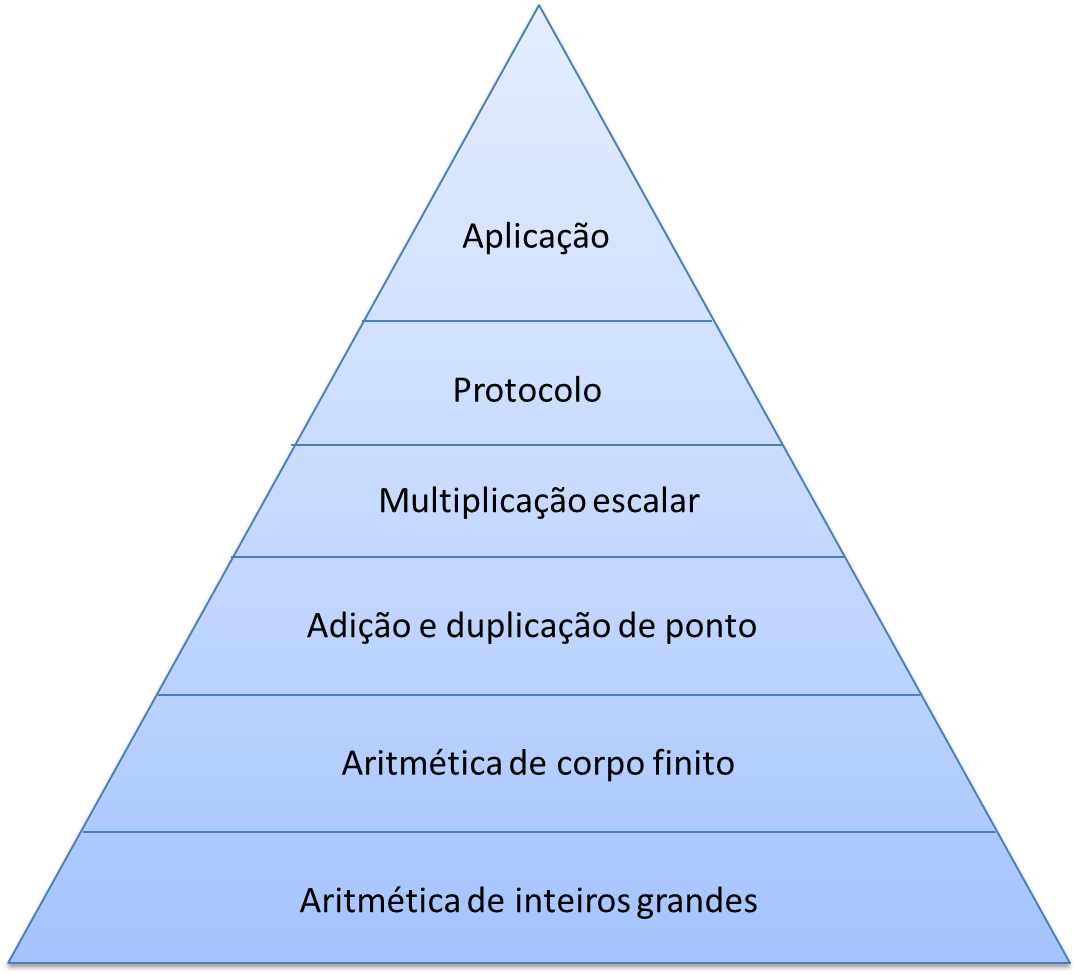
\includegraphics[width=0.7\textwidth]{figures/piramide_ECC.png}
	\caption{
		Pirâmide de implementação de criptografia baseada em curvas elípticas (ECC). Qualquer uma destas camadas pode ser vulnerável a ataques pode canais laterais.
	}
	%\vspace{.5mm}
	\label{fig:pyramid-ecc}
\end{figure}

A implementação de protocolos criptográficos baseados em curvas elípticas depende da existência de implementações de um conjunto de operações básicas, tais como: multiplicação de ponto por escalar, adição e duplicação de ponto, aritmética de corpo finito e aritmética de inteiros grandes. Protocolo criptográficos podem ser implementados a partir destas operações primitivas, os quais por sua vez possibilitam implementar um aplicação. A~\Cref{fig:pyramid-ecc} ilustra tais operações como níveis/camadas de uma pirâmide, onde a implementação de uma operação em uma camada depende apenas da existência de funcionalidades na camada imediatamente inferior\footnote{Operações adicionais podem ser necessárias para alguns protocolos, como a aritmética modular cujo módulo é o número de pontos da curva. Além disso, curvas elípticas definidas sobre corpos finitos binários dependem da aritmética em polinômios grandes.}.

A representação em pirâmide entretanto esconde a interdependência que existe entre as operações. Na prática, bibliotecas de primitivas e protocolos criptográficos há interação em todos os níveis da pirâmide, pois tais interações ou interdependências são relevantes para desempenho, e em alguns casos, segurança. 

Em uma implementação de uma dada aplicação, qualquer um dos níveis da pirâmide da figura acima pode estar vulnerável a ataques por canais laterais. Com relação ao canal de tempo, por exemplo, se uma operação não é de tempo constante com a relação à chave ou valores intermediários dependentes da chave, então todas as operações em níveis superiores à esta, bem como protocolo e aplicação vazam por diferenças potencialmente observáveis de tempo tais informações, as quais podem, a princípio, serem exploradas pelo atacante e portanto vulneráveis.

% (dentre aquelas entre a aritmética de inteiros grandes até a multiplicação escalar)

%\subsection{Transferência de chaves}
%\erick[inline]{TODO: Transferência da chave entre diferentes memórias}
%\erick[inline]{TODO: processamento da chave fora do algoritmo criptográfico. Ref. sobre um SCA bem sucedido deste tipo: Witteman, M. (2013). Secure Application Programming in the Presence of Side Channel Attacks.\cite{Witteman2013_PatternsAppsecSCA}. Autor demonstra um ataque à verificação de paridade da chave na biblioteca GnuPG.}

\subsection{Ataques de tempo e SPA ao algoritmo double-and-add-not-always}

\subsubsection{Ataque de tempo ao algoritmo double-and-add-not-always}
Considerando que o SPA de tempo se baseia na variação de tempo do algoritmo dependendo do valor da chave é possível realizar o ataque de tempo em algoritmos que não executam em tempo constante. Nesse caso, a maneira mas simples de observar uma implementação insegura é a presença de branchs condicionais. Um exemplo é no caso de um algoritmo possuir uma instrução de \textit{if} onde ele apenas executa as operações contidas nessa instrução dependendo dos \textit{bits} da chave privada.

Nesse contexto podemos observar um ataque de tempo aplicado a uma implementação do RSA por \cite{Kocher96}, esse foi o primeiro ataque de tempo proposto. O mesmo pode ser aplicado a implementações de curvas elípticas considerando que basicamente o atacante faz a análise do tempo de execução do algoritmo, tenta advinhar os \textit{bits} da chave e valida se o resultado está correto.

No trabalho de \cite{danger2013synthesis} é descrito um ataque à um implementação genérica de ECSM. O mesmo segue os seguintes passos: primeiramente o atacante coleta o tempo de execução de diferentes ECSMs com o mesmo escalar e diferentes pontos base. Para cada ECSM, ele simula a computação usando um simulador de software com exatamente a mesma implementação do chip alvo, "chutando" o valor do bit $i$ do escalar. 

Agora suponha, sem perda de generalidade, que a hipótese é de que o valor do \textit{bit} é $0$.  Ele separa os diferentes tempos de execução em dois conjuntos, $S_1$ e $S_2$. Caso uma redução é necessária ao final da execução o tempo obtido é armazenado em $S_2$, senão é armazenado em $S_1$. Após toda a execução é feita uma média dos tempos armazenados em $S_1$ e $S_2$, e se a diferença entre as médias for aproximadamente o tempo de execução da redução portanto a hipótese estava correta.

\begin{comment}
\erick[inline]{Lucas: ver o comentario no fonte. Converter comentario em texto}.

1.	Ataque SPA à alg. ECSM binário left-to-right (Dbl-and-Add not Always)
	a.	Se impl não é de tempo constante, então é possível realizar ataque de tempo.
		i.	P.ex., se usa if and else, então pode-se determinar a cada iteração qual bloco, if ou else, é tomado.
	b. O ataque de tempo em~\cite{Kocher96} ao RSA pode ser aplicado no contexto de ECC. Segue abaixo a ideia do ataque (baseada no survey de ~\cite{Danger2013}, Sec. 3.2.1).
	
	O atacante coleta o tempo de execução de diferentes ECSMs com o mesmo escalar e diferentes pontos base. Para cada ECSM, ele simula a computação usando um simulador de software com exatamente a mesma implementação do chip alvo, "chutando" o valor do bit $i$ do escalar. Suponha, sem perda de generalidade, que a hipótese é de que o valor do bit é 0.  Ele separa os diferentes tempos de execução em dois conjuntos, S_1 e S_2. Se, a iteração
	
	%TODO: CONT HERE
	

[Kocher96] Kocher, P.C.: Timing attacks on implementations of Diffie–
Hellman, RSA, DSS, and other systems. In: Proceedings of CRYPTO’96, LNCS, vol. 1109. Springer, Berlin, pp. 104–113
(1996)
\end{comment}

\subsubsection{Ataque SPA ao algoritmo double-and-add-not-always}
O algoritmo \textit{double-and-add-not-always} executa em tempo constante, contudo o ataque SPA (com ou sem power model) pode ser aplicado para distinguir os padrões no \textit{trace} das iterações com apenas DBL (onde o \textit{bit} da chave é igual à $0$) daquelas com DBL+ADD (com \textit{bit} da chave igual à $1$). Um ataque deste tipo segmenta/divide o \textit{trace} de potência de uma execução do ECSM em \textit{subtraces}, cada uma contendo uma operação de ponto (ADD ou DBL). 

Se o tempo de execução de uma operação de ADD for diferente do tempo de DBL, então o comprimento dos \textit{subtraces} revela onde estão os ADDs e consequentemente os bits do escalar. Se o tempo da operação ADD e o tempo da DBL forem iguais, e uma fórmula unificada para ADD and DBL é utilizada, então, se for aplicada correlação (coeficiente de correlação de Pearson) entre todos os pares de \textit{subtraces}, o resultado será que a correlação será mais alta para os pares de subtraces cuja operação correspondente é a mesma (i.e., (ADD,ADD) ou (DBL,DBL)), identificando portanto as operações de ponto e consequentemente os \textit{bits} do escalar.

Mesmo sendo que a implementação seja vulnerável a SPA é desejável que execute em tempo constante, o que cria uma base para a implementação de outras contramedidas. Portanto, é necessário observar que para executar o ataque SPA são requisitados equipamentos para medir a potência como um osciloscópio, além disso, o ataque por tempo possui simplicidade em comparação com SPA sendo que apenas é necessária a capacidade de verificar o tempo de execução do algoritmo e inserir entradas distintas.

\begin{comment}
\erick[inline]{Lucas: ver o comentario no fonte. Converter comentario em texto}.

b.	Se é de tempo constante, SPA (com ou sem power model) pode ser aplicado para distinguir os padrões no trace das iterações com apenas DBL (bit=0) daquelas com DBL+ADD (bit=1). Um ataque deste tipo segmenta/divide o trace de potencia de uma execucao do ECSM em subtraces, cada um contendo uma operacao de ponto (ADD ou DBL). Se as tempo(ADD) != tempo(DBL), então o comprimento dos subtraces revela onde estão os ADDs e consequentemente os bits do escalar. Se tempo(ADD) == tempo(DBL) e uma formula unificada para ADD and DBL é utilizada, então, se for aplicada correlação (coeficiente de correlacao de Pearson) entre todos os pares de subtraces, o resultado será que a correlação será mais alta para os pares de subtraces cuja operação correspondente é a mesma (i.e., (ADD,ADD) ou (DBL,DBL)), identificando portanto as operações de ponto e consequentemente os bits do escalar.
\end{comment}

%TODO 2. Argumentar que é fortemente desejável que as implementações sejam de tempo constante, de modo a ser uma base para a implementação das outra contramedidas para power analysis.

\subsection{Double-and-add-always algorithm of Coron~\cite{Coron1999}}

\begin{comment}
\erick[inline]{Lucas: traduzir esta secao}
\end{comment}

O algoritmo {\it double-and-add-always} de \cite{Coron1999} (Algoritmo 11) utiliza uma adição de ponto falsa conhecida como \textit{dummy point addition} quando o \textit{bit} escalar $k_i$ é $0$, tornando a sequência de operações computadas durante a multiplicação escalar independente do valor do escalar.

\begin{algorithm}[h] %\scriptsize %\footnotesize
	\caption{\small{\textit{Double-and-add always} algorithm resistant against SPA}}
	\label{Double-and-add-Coron}
	\begin{algorithmic}[1]
		\REQUIRE  Point $\textbf{P} \in E(\mathbb{F}_q),$ $k=(k_{n-1},\ldots,k_1,k_0)_2 \in \mathbb{N}$
		\ENSURE  $Q=[k] \cdot P$\\
		\STATE $R_0\leftarrow P_{\infty}$   \\
		\FOR{$i$ \textbf{from} $n-1$ \textbf{to} $0$} 
		\STATE $R_0\leftarrow 2R_0$  \\
		\STATE $R_1\leftarrow R_0+P$\\ \label{Paso_R_1_Double-and-add-Coron}
		\STATE $R_0\leftarrow R_{k_i}$\label{Step5Double-and-add-Coron} \\
		\ENDFOR
		\STATE return $R_0$\\
	\end{algorithmic}
\end{algorithm}

Portanto o adversário não consegue, em princípio, advinhar o valor do \textit{bit} $k_i$ por SPA. Uma desvantagem desse método é a sua baixa eficiência. Ele requer $nA + nD$ operações no corpo, um aumento de $33\%$ nas operações do corpo em comparação a versão desprotegida binária do algoritmo \textit{left-to-right}.

\subsubsection{Fouque and Valette's Doubling Attack \cite{CHES:FouVal03}}\label{Fouque-Valette-DoublingAttack}
O ataque de duplicação de Fouque-Valette~\cite{CHES:FouVal03} é baseado no fato de que é possível detectar se dois valores intermediários são iguais quando o algoritmo calcula a multiplicação escalar para pontos escolhidos $P$ e $2P$. Diversos algoritmos protegidos contra SPA são vulneráveis ao ataque d eFouque e Valette's, como o algoritmo clássico \textit{left-to-right} binário, incluindo as variações do mesmo, como o \textit{double-and-add-always} de Coron.

No algoritmo de Coron \textit{double-and-add-always}, algoritmo (Algoritmo~\ref{Double-and-add-Coron}), a soma parcial é calculada da seguinte maneira: $S_m(P) = \sum_{i=1}^{m}k_{n-i}2^{m-i} P=\sum_{i=1}^{m-1}k_{n-i}2^{m-1-i}(2P)+k_{n-m}P= S_{m-1}(2P)+k_{n-m}P$. Então o resultado intermediário do algoritmo no passo $m$ quando a entrada for $P$ será igual ao resultado intermediário no passo $m-1$ quando a entrada for $2P$, se e somente se, $k_{n-m} = 0$. Portanto, um atacante pode obter o escalar secreto comparando a computação de duplicação no passo $m+1$ para $P$ e no passo $m$ para $2P$ para recuperar o bit $k_{n-m}$. Se ambas as computações forem idênticas, $k_{n-m} = 0$, senão $k_{n-m} = 1$. Isso mostrou que com apenas duas requisições de multiplicação escalar escolhidas pelo atacante, é possível recuperar todos os \textit{bits} do escalar.~\footnote{O atacante coleta um traço de energia para a computação de $kP$ e um para a computação de $k(2P)$. Para cada iteração $m=1,...,n$ ele executa o ataque como descrito e encontra $k_{n-m}$.}

\begin{comment}
The doubling attack of Fouque-Valette~\cite{CHES:FouVal03} is based on the fact that it is possible to detect if two intermediate values are equal when the algorithm computes the scalar multiplication for points chosen points $P$ and $2P.$ Several algorithms protected against SPA are vulnerable to Fouque and Valette's attack, such as the classic binary left-to-right algorithm, including those derived from it, such as Coron's double-and-add-always algorithm.

%In ~\textit{double-and-add-always} algorithm (Algorithm~\ref{Double-and-add-Coron}), the partial sums are computed as follows: $S_k(P) = \sum_{i=0}^{k}d_{n-i}2^{k-i} P=\sum_{i=0}^{k-1}d_{n-i}2^{k-1-i}(2P)+d_{n-k}P= S_{k-1}(2P)+d_{n-k}P$. So, the intermediate result of the algorithm at step $k$ when given input $P$ will be equal to the intermediate result at step $k-1$ when given input $2P$, if and only if, $d_{n-k}=0$. Therefore, an attacker can obtain the secret scalar by comparing the doubling computation at step $k+1$ for $P$ and at step $k$ for $2P$ to recover the bit $d_{n-k}.$ If both computations are identical, $d_{n-k}=0$, otherwise $d_{n-k}=1$.
In Coron's double-and-add-always algorithm (Algorithm~\ref{Double-and-add-Coron}), the partial sums are computed as follows: $S_m(P) = \sum_{i=1}^{m}k_{n-i}2^{m-i} P=\sum_{i=1}^{m-1}k_{n-i}2^{m-1-i}(2P)+k_{n-m}P= S_{m-1}(2P)+k_{n-m}P$. So, the intermediate result of the algorithm at step $m$ when given input $P$ will be equal to the intermediate result at step $m-1$ when given input $2P$, if and only if, $k_{n-m}=0$. Therefore, an attacker can obtain the secret scalar by comparing the doubling computation at step $m+1$ for $P$ and at step $m$ for $2P$ to recover the bit $k_{n-m}.$ If both computations are identical, $k_{n-m}=0$, otherwise $k_{n-m}=1$. It has been shown that with only two scalar multiplication requests chosen by the attacker, it is possible to recover all the bits of the scalar.~\footnote{The attacker collects one power trace for the computation of $kP$ and one for the computation of $k(2P)$. For each iteration $m=1,...,n$, he runs the attack as described and finds $k_{n-m}$.}
%%\vspace{-0.5cm}
\end{comment}


\subsection{Contramedidas}

% TODO: apresentar uma contramedida de cada vez entre subseções com ataques, mostrando como ela protege contra um determinado ataque.

\begin{comment} % === CONTRAMEDIDAS ===
	a.	CM1 - Scalar Randomization (SR)
	b.	CM2 - Proj. Coord. Randomization and Re-randomization (CRR)
	c.	CM3 - Point Blinding (PB) 
	d.	CM4 – Scalar Splitting (SS)
\end{comment}

\subsubsection{Scalar Randomization (SR)}
Essa contramedida é aplicada no início da multiplicação escalar, e é executada da seguinte maneira:
\begin{itemize}
    \item Aleatoriamente selecione $r\in_R \{0,1\}^n$, para um pequeno $n$. $n=32$ é um parâmetro razoável no quesito do \textit{trade-off} entre segurnaça/eficiência;
    \item Calcule $k' \rcv k + r |E|$;
    \item Utilize $k'$ no lugar de $k$.
\end{itemize}

O custo da aplicação dessa contramedida está ligado à geração dos \textit{bits} pseudo-aleatório, $n$ iterações da ECMS, as adições e multiplicações para calcular $k'$ e $n$ \textit{bits} da SRAM. Já no quesito eficiência é necessário verificar que é vulnerável a ataques de template online (OTA) \cite{BatinaChmielewski2014}, entre outros. 

\begin{comment}
	%	\begin{itemize}
	%\item 
	At the beginning of the scalar multiplication:
	\begin{enumerate}
		\item Randomly select $r\in_R \{0,1\}^n$, for a small $n$. $n=32$ seems to be a reasonable security/efficiency trade-off.
		\item Compute $k' \rcv k + r |E|$.
		\item Use $k'$ in place of $k$.
	\end{enumerate}
	
	%\item 
	\underline{Cost}: generate $n$ (pseudo-)random bits, $n$ iterations to the ECSM, MULs and ADDs to compute $k'$, $n$ bits of SRAM.\\
	%\item 
	
	\underline{Effectiveness}: vulnerable to Online Template Attacks (OTA) {[Batina,2014]}, among others.
	%	\end{itemize}

\end{comment}

\subsubsection{Projective Coordinates (Re-)Randomization (CR)~\cite{Coron1999}}
As coordenadas projetivas usadas em Montgomery Ladder são $(X : Z)$. Os passos para aplicar essa contramedida são:
\begin{itemize}
    \item Gerar um valor pseudo-aleatório $\lambda \mathbb{F}_p \backslash \{0\}$;
    \item Calcule $Z_2 \rcv \lambda$ and $X_2 \rcv u \cdot \lambda$, onde $u$ é a coordenada $x$ do ponto $P$ da entrada;
    \item Utilize $P'=(X_2:Z_2)$ no lugar de $P$.
\end{itemize}

Existe um custo de geração de $\ceil{log_2(p)}$ \textit{bits} aleatórios. Além disso, algumas vantagens ligadas a essa randomização das coordenadas como por exemplo a resistência à ataques online de template \cite{BatinaChmielewski2014}, pode ser aplicada para as curvas de Edwards, \textit{twisted} Edwards e Montgomery. Por fim, a cada iteração do método de ECSM ela pode ser aplicada, sendo apenas necessária a coordenada $x$ no caso de Montgomery Ladder.


\begin{comment}
\erick[inline]{Lucas: traduzir e escrever em texto corrido. Descrito para o caso de Montgomery Ladder somente com a coordenada $x$}

Original projective coordinates used in Mont Ladder: $(X:Z)$.\\
In the beginning of the ECSM, do:
\begin{enumerate}
	\item Generate random $\lambda \mathbb{F}_p \backslash \{0\}$.
	\item Do $Z_2 \rcv \lambda$ and $X_2 \rcv u \cdot \lambda$, where $u$ is the $x$-coordinate of input point $P$.
	\item Use $P'=(X_2:Z_2)$ in place of $P$.
\end{enumerate}	
\underline{Cost}: generation of $\ceil{log_2(p)}$ random bits, 1 M.\\
\underline{Effectiveness}: 
\begin{itemize}
	\item Resistant to Online Template Attacks~\cite{BatinaChmielewski2014}.
	\item Can also be applied to Edwards, twisted Edwards and Montgomery curves.
	\item Can also be used at every ECSM iteration (re-randomization).
\end{itemize}
\end{comment}

\subsubsection{Point Blinding (PB)~\cite{Coron1999}}
Essa contramedida pode ser aplicada, antes da primeira multiplicação escalar, seguindos os passos apresentados a seguir: 
\begin{itemize}
    \item Com o escalar $k$ é necessário gerar um ponto aleatório $R$ no subgrupo;
    \item Pre-calcule e armazene $S = [k]R$;
    \item No início de cada operação escalar calcule $T \rcv P + R$ e $Q \rcv [k] T$;
    \item Atualize $R$ e $S$ da seguinte maneira:
    \begin{itemize}
        \item $R \rcv (-1)^t 2R$;
        \item $S \rcv (-1)^t 2S$;
        \item $t \in \{0,1\}$ escolhido de forma aleatória.
    \end{itemize}
    \item Retorne $W = Q - S$.
\end{itemize}

O custo encontrado nessa contramedida é de 2 ECADD, 2 ECDBL, e memória SRAM para valores temporários. Provavelmente também é utilizada memória não volátil para armazenar $R$ e $S$. \textit{Point Blinding} protege contra SVA horizontal \cite{MurdicaGuilley2012}, RPA \cite{Goubin2003}, e ZPA \cite{AkishitaTakagi2003}, mas é vulnerável à OTA \cite{BatinaChmielewski2014}

\begin{comment}
\erick[inline]{Lucas: traduzir e escrever em texto corrido.}

Before the first scalar multiplication with scalar $k$:
\begin{itemize}
	\item Generate random point $R$ in the subgroup.
	\item Precompute and store $S = [k]R$.
\end{itemize}

At the beginning of each scalar multiplication:
\begin{itemize}
	\item Compute $T \rcv P + R$.
	\item Compute $Q \rcv [k] T$.
	\item Update $R$ and $S$: $R \rcv (-1)^t 2R$ and $S \rcv (-1)^t 2S$, $t \in \{0,1\}$ is randomly chosen.
	\item Return $W = Q - S$.
\end{itemize}

\noindent  \underline{Cost}: 2 ECADD, 2 ECDBL, SRAM memory for temps. Probably also writable non-volatile memory to store $R$ and $S$.\\
\noindent \underline{Effectiveness}: protects against horizontal SVA~\cite{MurdicaGuilley2012}, RPA~\cite{Goubin2003} and ZPA\cite{AkishitaTakagi2003}. Vulnerable to OTA~\cite{BatinaChmielewski2014}.
\end{comment}


% Definitions ==========================================================
% RPA = Refined Power Analysis. Intermed. point with one of the coords zero.
% ZPA = Zero Value Point Attacks. Itermed. value (e.g., field elem), is zero
% SVA = Same Value Analysis. Generalization of ZPA when the intermediate value has a special value (not necessarily 0), that can be easily distinguished.
%==========================================================
\subsubsection{Scalar Splitting (SS)~\cite{ClavierJoye2001}}
A aplicação dessa contramedida segue, sendo $k$ o escalar original de $n$ \textit{bits}, os seguintes passos:
\begin{itemize}
    \item Gere um inteiro $k_1 < k$ aleatoriamente
    \item Faça $k_2\rcv k - k_1$
    \item Calcule $Q\rcv [k_1]P$
    \item $T\rcv[k_2]P$ 
    \item $R\rcv Q + T$. 
\end{itemize}

O custo dessa contramedida é a execução de 1 ECSM de $n$ \textit{bits} e 1 ECADD. O mesmo pode ser reduzido se for empregado truque de Shamir para multiplicação escalar dupla (versão regular)~\cite{CietJoye2003}. A eficácia está ligada a resistência aos ataques TA, SPA clássico e CPA clássico. As variantes dessa contramedida são: Euclidean splitting~\cite{CietJoye2003} e \textit{multiplicative splitting}~\cite{TrichinaBelleza2003}, ambas com a mesma eficácia da versão original, também conhecida como \textit{additive splitting}.

\begin{comment} % === Ataques SCA contra ECC devem ser do tipo single-trace  ===
5.	Explicar porque no contexto de PKC (RSA e ECC) não fazem sentido ataques que envolvem mais de um trace, como p.ex., DPA.
\end{comment}


\begin{comment}  % === ESTRUTURA ORIGINAL ===
\subsubsection{Ataques baseados em templates}
\subsubsection{Ataques horizontais baseados em cross-correlation}
\subsubsection{Ataques horizontais não-supervisionados baseados em clustering}

\subsubsection{Aplicação de contramedidas em algoritmo esquerda para direita inseguro}
\subsubsection{Implementações de tempo constante}
\subsubsection{Implementações resistentes ao SPA}
\subsubsection{Impacto das contramedidas no desempenho}

\subsection{Eficácia de implementação de tempo constante}
\subsubsection{Outros métodos para inviabilizar ataques por tempo}
\end{comment}

%\subsection{Ataque SPA à alg. Montgomery Ladder com SR}
%\erick[inline]{Descrever idéia de online template attack (OTA)~\cite{BatinaChmielewski2014}}

%\subsection{Ataque SPA à alg. ECSM atômico com SR}
%\erick[inline]{Explicar como online template attack (OTA)~\cite{BatinaChmielewski2014} pode ser aplicado neste caso}

%\subsection{Ataque template SPA à alg. Montgomery Ladder com SR + CRR}
%\erick[inline]{Copy-and-paste de partes do meu paper no SAC 2016.}

\subsection{Ataques Horizontais (HA)}
% source: RSC-intern-plan

Ataques horizontais (HA) são uma metodologia para ataques por canal lateral cujos alvos são as principais operações criptográficas em protocolos baseados em RSA e ECC, a exponenciação modular e a multiplicação escalar, respectivamente. Em teoria, tais ataques permitem recuperar os bits do expoente/escalar secreto através da análise de traces individuais, isto é, apenas um único trace obtido do alvo é suficiente, portanto são eficazes contra implementações protegidas por contramedidas como SR, CR, PB e SS.

Um requisito básico dos ataques horizontais é o conhecimento do algoritmo de multiplicação escalar. De posse de tal informação, o atacante pode escolher, dentre outros, os seguintes métodos ou \textit{distinguishers}: correlation analysis, collision-correlation analysis e cluster analysis.     %SPA, distancia euclidiana, horizontal correlation analysis, horizontal collision-correlation, horizontal cross-correlation ou clustering.
% TODO: definir distinguisher

% Correlation analysis
O método de correlation analysis~\cite{Clavier2010} segue o mesmo princípio da análise de potência por correlação (CPA)\footnote{\textit{Correlation power analysis}.} aplicada a um conjunto de traces, na configuração vertical. A diferença para o contexto horizontal é de que um único trace é dividido em vários segmentos e para cada um destes segmentos um valor intermediário hipotético é atribuído, com respeito a um chute sobre o valor da chave. A correlação entre amostra e valor hipotético é calculada do mesmo modo que CPA, e os modelos de vazamentos usualmente utilizados são o peso de Hamming e a distância de Hamming. Este método funciona contra implementações protegidas somente com SR, ou quando CR é também aplicada mas o parâmetro aleatório utilizado é curto, e ataques por força bruta ao valor de tal parâmetro são viáveis.

% Collision-correlation analysis
O método de collision-correlation analysis~\cite{Bauer2013_CTRSA, Bauer2013, Clavier2012_Indocrypt, WittemanWoundenbergMenari2011, Walter2001_Ches} computa a correlação ou distância euclideana entre diferentes segmentos de um trace. O objetivo principal é identificar a ocorrência de um mesmo dado intermediário em diferentes partes de um trace, e com isso derivar os bits do escalar secreto. Para tanto, o atacante deve ter conhecimento sobre o algoritmo de ECSM empregado. Em teoria, este método é viável contra implementações envolvendo combinações de contramedidas clássicas.

% Desafios / limitações
A maioria das formas de ataques horizontais requer pré-processamento avançado dos traces, caracterização e avaliação de vazamento antes da aplicação de distinguishers. Os principais problemas da abordagem horizontal são de que extrair o vazamento a partir de um único trace tipicamente apresenta fortes limitações e desafios, como o alto nível de ruído e a indisponibilidade de amostras rotuladas. Em particular, métodos de avaliação de vazamento, como o TVLA~\cite{Goodwill2011}, requerem amostras rotuladas e isso não é possível quando a contramedida SR é aplicada.

% Cluster analysis
Métodos baseados em aprendizado não supervisionado, mais especificamente aqueles baseados em clustering, foram recentemente aplicados para resolver tais limitações e têm se mostrado capazes de produzir resultados práticos. Heyszl et al~\cite{Heyszl2013} propõem aplicar classificação por clustering à um único trace para possibilitar a identificação de classes específicas de operações; este método funciona bem para medições com baixo ruído e requer uma estação de EM composta de múltiplas sondas. Em Perin et al's~\cite{Perin2014}, os autores consideram uma abordagem heurística baseada na diferença de médias para a seleção de pontos de interesse. Além disso, ambas soluções usam um único trace como entrada para a etapa de avaliação de vazamento, o qual pode ter sido muito afetado por uma grande quantidade de ruído. Perin e Chmielewski~\cite{PerinChmielewski2015} fornecem uma metodologia para ataques horizontais baseados em clustering que foca em corrigir as deficiências dos trabalhos mencionados anteriormente.

\subsection{Ataque HCA à alg. Montgomery Ladder c/ SR + CRR}
% Meu projeto na RSC, artigos Perin 2014 e 2015.

\subsubsection{Preparação: filtragem, segmentação e alinhamento}
% filtragem dos traces
% segmentação dos traces em iterações da ECSM
% alinhamento dos subtraces

Em ataques horizontais, devido a problemas como o alto nível de ruído presente em um trace, fenômenos como clock drift\footnote{Clock drift ou clock jitter é o desvio do sinal de clock real em relação ao sinal verdadeiramente periódico de referência. Devido ao clock drift, o sinal de clock real não é periódico, mas sim aproximadamente periódico.} e variações no tempo em que dispositivo de medição (osciloscópio) inicia a medição após o recebimento do sinal de trigger (\textit{trigger jitter}), é fundamental o preprocessamento dos traces medidos antes de se iniciar a análise, particularmente as operações de filtragem, segmentação e alinhamento.

\noindent \textbf{Filtragem.} A \Cref{fig:tracesFiltering} mostra um trace não filtrado e o mesmo trace após aplicação de filtro baixa, onde pode-se identificar com mais clareza características do sinal, como periodicidade e amplitude, bem como as rodadas ou iterações. É recomendável que filtros analógicos sejam aplicados, sempre que possível, de modo que o sinal que é digitalizado pelo osciloscópio contém apenas as frequências desejadas, permitindo o uso da menor resolução (range) vertical suportada pelo dispositivo, o que pode não ocorrer caso picos em frequências indesejadas estejam presentes.

\begin{figure}
	\label{fig:tracesFiltering}
	\centering
	\begin{subfigure}[b]{0.8\textwidth}
		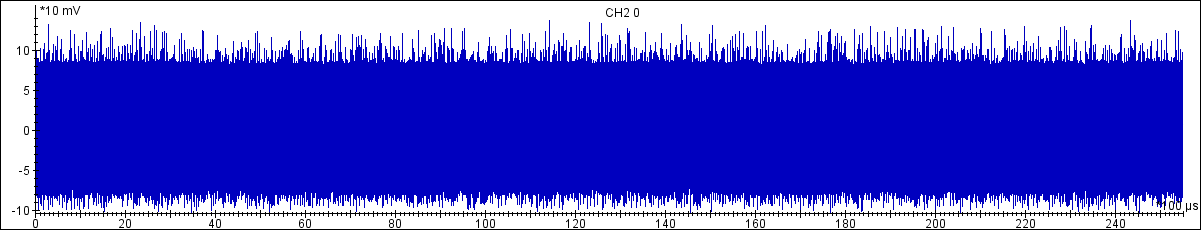
\includegraphics[width=1\linewidth]{figures/Trace_EM___MontLadder___CPU_168MHz___SR_1GHz___32MS___UNFiltered.png}
		\caption{}
		\label{fig:traceUnfiltered} 
	\end{subfigure}
	
	\begin{subfigure}[b]{0.8\textwidth}
		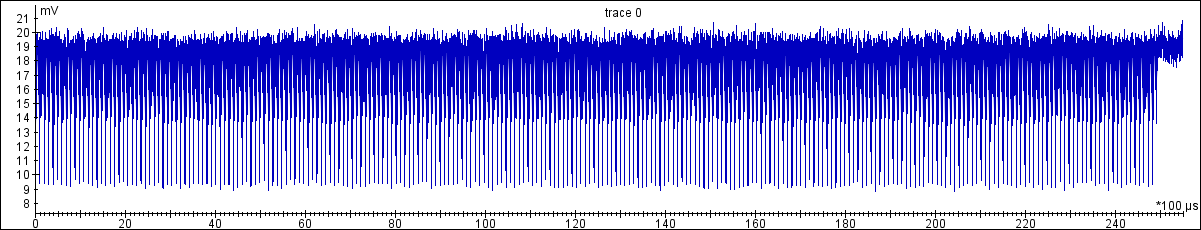
\includegraphics[width=1\linewidth]{figures/Trace_EM___MontLadder___CPU_168MHz___SR_1GHz___32MS___Filtered.png}
		\caption{}
		\label{fig:filtered}
	\end{subfigure}	

	\begin{subfigure}[b]{0.8\textwidth}
		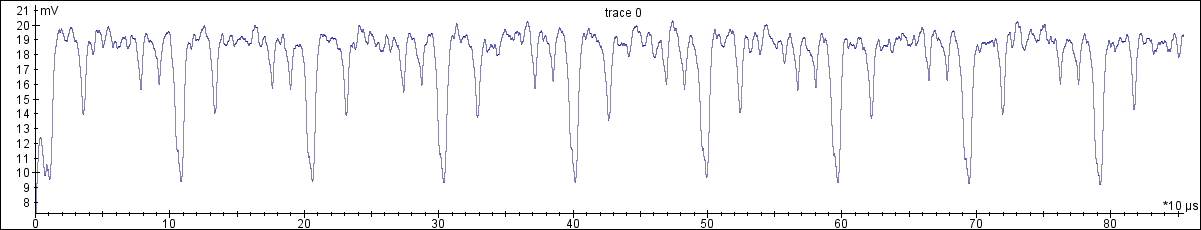
\includegraphics[width=1\linewidth]{figures/Trace_EM___MontLadder___CPU_168MHz___SR_1GHz___32MS___Filtered___Zoom_in.png}
		\caption{}
		\label{fig:filteredZoomIn}
	\end{subfigure}
	
	\caption{Um trace de radiação eletromagnética de uma execução de ECSM com algoritmo Montgomery Ladder: original não filtrado (a), após aplicação de filtro baixa (b) e zoom no início deste último (c).}	
\end{figure}

\noindent \textbf{Segmentação.} Os traces de potência medidos tipicamente correspondem à execução completa da operação criptográfica, sendo assim são contíguos e contêm todas as rodadas (rounds) ou sub-operações executadas; no contexto da multiplicação escalar, as rodadas são as $n$ iterações do laço do algoritmo de multiplicação escalar implementado. Tais traces devem ser primeiramente segmentados em iterações, de modo que um conjunto de $n$ subtraces é obtido, cada um contendo as amostras correspondentes à respectiva iteração.

\noindent Tal segmentação pode ser realizada de diversas maneiras. Um método ingênuo é identificar os índices das amostras de início e fim da execução do laço da ECSM, e então dividir este segmento em $n$ segmentos de igual (ou quase igual) comprimento, cada qual correspondendo a uma iteração. Tal método apresenta dois problemas, o primeiro é de que em geral é difícil identificar as amostras de início e fim; o segundo é que o comprimento dos segmentos das iterações podem variar devido ao clock jitter. Um método mais robusto, que ameniza tais dificuldades, é aplicar um filtro passa baixa forte, de modo a identificar segmentos do trace que se repetem de uma iteração para outra; localizar então picos nestes segmentos cuja distância entre si é aproximadamente a mesma (Tal distância é o valor aproximado do comprimento daquela iteração) e por fim cortar o trace original utilizando tais comprimentos como referência. No entanto, devido às dificuldades anteriormente mencionadas, é provável que a segmentação obtida não seja perfeita, e portanto amostras do início de um iteração poderão estar presentes no trace da iteração anterior, bem como amostras do fim de um iteração poderão estar no início do trace da iteração seguinte e analogamente com relação à primeira e a última iterações e as partes do trace externas ao laço da ECSM.

\noindent \textbf{Alinhamento.} Dado que a segmentação provavelmente não será perfeita, uma operação aritmética realizada no intervalo de amostras $tr_i[s..e]$ no trace da iteração $i$ muito provavelmente ocorrerá em um itervalo diferente $tr_j[s'..e']$ no trace da iteração $j$. Logo, é necessário alinhar todos os subtraces de iterações da ECSM. A \Cref{fig:traceAlignment} mostra alguns traces resultantes da segmentação antes e após alinhamento estático por correlação. Diversos algoritmos para alinhamento de traces para SCA são propostos na literatura, dentre eles o alinhamento estático e o alinhamento elástico~\cite{WoudenbergWittemanBakker2011}. O alinhamento estático é um método simples que consiste, a grosso modo, em escolher um trace de referência e deslizar incrementalmente o trace a ser alinhado sobre o de referência e computar a distância entre eles de acordo com alguma métrica, p.ex. o coeficiente de correlação de Pearson; após deslizar por um dado número de posições, dentro de uma janela, considera-se que o trace estará alinhado se for deslocado (\textit{shifted}) até a posição cuja distância foi mínima.

\begin{figure}
	\label{fig:traceAlignment}
	\centering
	\begin{subfigure}[b]{0.8\textwidth}
		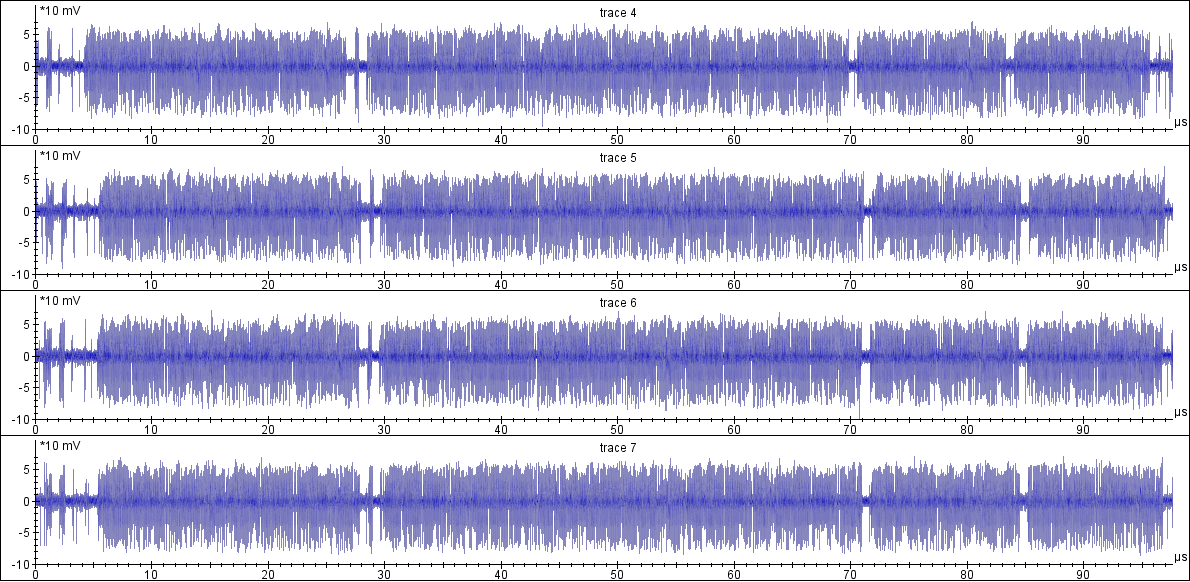
\includegraphics[width=1\linewidth]{figures/Traces_EM___MontLadder___CPU_168MHz___SR_1GHz___28MS___Misaligned.png}
		\caption{}
		\label{fig:misaligned} 
	\end{subfigure}
	
	\begin{subfigure}[b]{0.8\textwidth}
		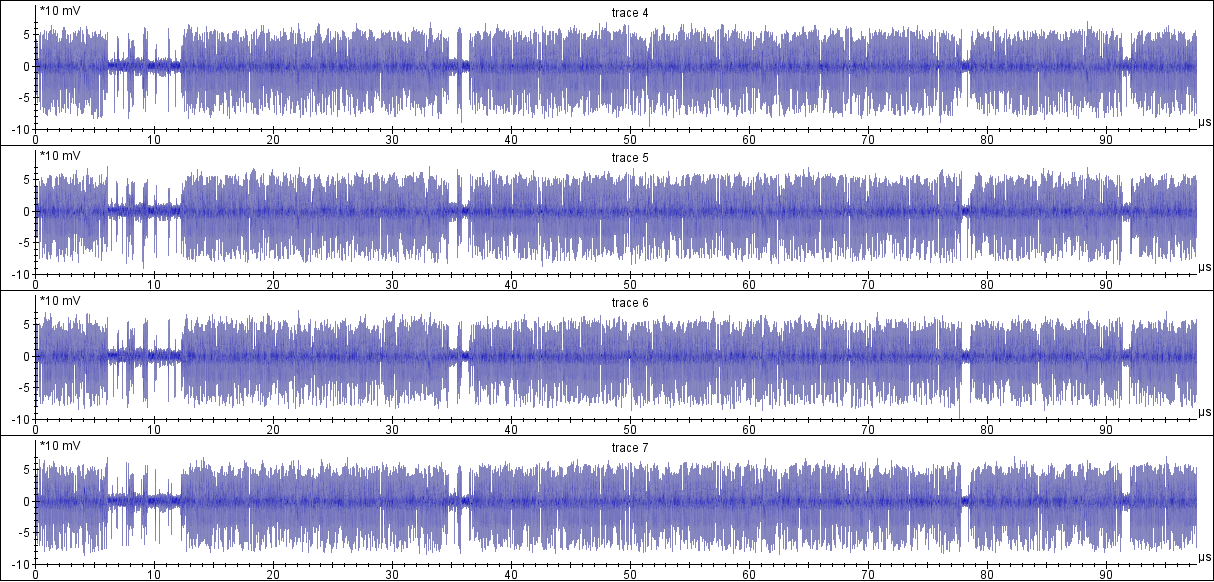
\includegraphics[width=1\linewidth]{figures/Traces_EM___MontLadder___CPU_168MHz___SR_1GHz___28MS___Aligned.png}
		\caption{}
		\label{fig:aligned}
	\end{subfigure}	
	
	\caption{Traces de iterações da ECSM: logo após segmentação, desalinhados (a); e após alinhamento (b).}
\end{figure}

\subsubsection{Algoritmos para clustering}
% Citar que K-Means, Fuzzy KMeans e Expectation-Maximization já foram empregados para este propósito, e apresentaram resultados semelhantes.

Em SCA, métodos de análise baseados em aprendizado de máquina, tais como Support Vector Machines~\cite{Bartkewitz2013}, Random forests~\cite{Lerman2014RFandSOM}, análise de séries temporais~\cite{Lerman2013} e análise nebulosa (\textit{Fuzzy analysis})~\cite{SaeediKong2014}  tem sido recentemente empregados como uma alternativa ao método de template attack no contexto de ataques~\textit{profiled}, em particular quando a distribuição das amostras difere muito da distribuição gaussiana; e também no contexto de ataques não profiled, através da utilização de algoritmos de clustering não supervisionados.

%No contexto de HCA, algoritmos de aprendizado não supervisionado baseados em clustering obtiveram sucesso em implementações \erick{continuar e citar}.

Dentre os algoritmos para clustering empregados com sucesso no contexto de ataques horizontais estão o K-Means~\cite{Forgy1965KMeans, Lloyd1982KMeans}, Fuzzy K-Means~\cite{Dunn1973FuzzyKMeans} e o Expectation-Maximization (EM)~\cite{DempsterLairdRubin1977EMAlg}. O K-Means é um algoritmo de clustering rígido, isto é, cada instância (uma amostra, no contexto de HCA) é atribuída (rotulada) a um único cluster. Fuzzy K-Means and EM, por outro lado, são algoritmos de clustering suaves (\textit{soft}), pois tem como saída uma matriz de probabilidade de associação onde à cada instância está associado o grau de vínculo desta com cada um dos clusters. Referimos o leitor aos livros sobre aprendizado de máquina~\cite{Alpaydin2014, WittenFrank2011, Han2011, Bishop2007, DudaHartStork2001} para descrições destes algoritmos e variantes.

% wONT_DO: O Explicar como o algoritmo Expectation Maximization funciona.

\subsubsection{Análise com chave conhecida}
% aplica-se clustering 1D no conjunto de amostras em um dado sample index

A análise com chave conhecida consiste em determinar os pontos de interesse, isto é, os índices de amostra, onde o vazamento é mais forte, com base no conhecimento da chave. Devido à necessidade de conhecimento do valor chave/escalar, tal análise é empregada somente na fase de teste do ataque HCA, para determinar, por exemplo, quantos traces são necessários como entrada para a avaliação de vazamento, de um dado dispositivo, de modo que os pontos de interesse obtidos por aquela correspondam aos previstos e sabidamente relevantes obtidos pela análise com chave conhecida.

Tal análise consiste em aplicar o algoritmo de clusterização no conjunto de amostras presentes em um dado índice de amostra ($m$), obtendo-se dois grupos de amostras: o primeiro grupo corresponde às amostras rotuladas com o valor b ($b\in \{0,1\}$, mas não se sabe se 0 ou 1) e o segundo grupo corresponde ao valor oposto $\bar{b}$. 

O conhecimento da chave é utilizado para determinar quantos bits tiveram o seu valor corretamente identificado no agrupamento. Como não se sabe o valor de $b$, isto é, o rótulo de cada grupo, o seguinte procedimento é adotado. Toma-se $b=0$ e conta-se o número de bits corretamente identificados ($n_c$); o valor $n - n_c$ ($n$ é o comprimento em bits do escalar) é então o número de bits corretamente identificados caso a rotulação esteja errada (isto é, o correto é $b=1$). Finalmente, considera-se $max\{n_c, n - n_c\}$ o número de bits corretamente identificados.

Este procedimento acima descrito é repetido para todos os índices de amostra, e o resultado são os pontos em que o vazamento de bits da chave é mais intenso. A ordenação destes pontos em ordem decrescente do número de bits corretamente identificados fornece os pontos de interesse.

\erick[inline]{Figura com clusterizacao obtida pelo EM e os rotulos corretos (com erros destacados, se possível.}

\subsubsection{Avaliação de vazamento} % leakage assessment
% aplica-se clustering 1D no conjunto de amostras em um dado sample index. Um grande traceset é necessário.
% a seguir é aplicada uma das funções "distinguisher": DoM, MIA, SOSD ou SOST.

Técnicas de avaliação de vazamento determinam se um dispositivo criptográfico está vazando informação por canal lateral, com base em método estatístico e um modelo de vazamento. 
Em~\cite{Meynard2011} os autores testaram informação mútua (MIA)\footnote{Mutual Information Analysis.} como um método para localizar vazamento no domínio da frequência e, consequentemente, encontrar as bandas de frequência no traces de EM do RSA em que as diferenças entre quadrados e multiplicações são maiores. O Welch $t$-test é um outro método estatístico que pode ser empregado para este fim, p.ex., em metodologias como a TVLA (cf.~\Cref{sec-tvla}). Os autores de~\cite{MatherOswaldBandenburg2013} demonstraram como empregar $t$-test e MIA para localizar vazamento no domínio do tempo.

No escopo de ataques horizontais, tais métodos são empregados sem que haja conhecimento do valor da chave secreta ou de números aleatórios gerados e/ou usados pelo dispositivo. Portanto, são aplicáveis em um cenário realista onde o adversário não tem qualquer controle (escrita ou leitura) da chave dispositivo ou outra informação secreta, em particular quando contramedidas como SR e CRR são aplicadas e não podem ser desabilitadas. Os pontos em que o vazamento é mais intenso, obtidos pela aplicação de um método para análise de vazamento, são tomados como pontos de interesse (POI). O valor das amostras em tais pontos são posteriormente utilizados na fase de ataque para recuperação da chave.

O método de análise de vazamento proposto em~\cite{PerinChmielewski2015} demonstra como múltiplos traces podem ser combinados para a avaliação de vazamento, no contexto de ataques horizontais ao RSA. Tal método é baseado em clustering e funciona mesmo se o dispositivo emprega qualquer combinação das contramedidas clássicas aplicadas à implementações da exponenciação modular: exponent blinding, message or modulus randomization.\footnote{Exponent blinding e message randomization são equivalentes às contramedidas SR e CRR para ECC, respectivamente}

\subsubsection{Avaliação de vazamento baseada em clustering}

Descrevemos nesta Subseção como o método de análise de vazamento de Perin e Chmielewski~\cite{PerinChmielewski2015} pode adaptado à uma implementação do algoritmo Montgomery Ladder para multiplicação escalar. Supomos que deseja-se identificar o valor do bit do escalar utilizado em cada iteração do laço principal deste algoritmo através de algum vazamento direto ou indireto deste valor. Sejam $n_0$ e $n_1$ o número de bits 0 e 1 em um trace. A razão $n_0/n_1$ é aproximadamente constante, tendendo a $1.0$, partindo da premissa de que o bits do escalar são gerados aleatoriamente. Devido à contramedida SR, o escalar efetivamente utilizado no laço da ECSM varia entre uma execução e outra da ECSM, e portanto difere de um trace para outro.

O método tem as seguintes premissas sobre o modelo de vazamento:
\begin{itemize}
	\item \textbf{Premissa 1}: em um trace $i$, o valor médio para o conjunto de amostras em um índice $m$ que correspondem às iterações cujo bit são 0 ou 1 são, respectivamente, $\mu_0^i + \gamma_0^i$ e $\mu_1^i + \gamma_1^i$, onde $\gamma_k^i$ é um ruído aleatório com distribuição normal, $k=0,1$.
	\item \textbf{Premissa 2}: para todos os traces $i$, as médias $\mu_0^i$ e $\mu_1^i$ são constantes.
\end{itemize}

Seja um trace $i$ e as amostras localizadas em um índice $m$ deste trace. A saída do algoritmo de clustering quando aplicado a este conjunto de amostras são dois centróides, $c_{0,m}$ e $c_{1,m}$ e dois clusters de amostras $\{g_{0,m}\}$ e $\{g_{1,m}\}$ contendo $p_{0,m}$ e $p_{1,m}$ elementos cada, respectivamente, tal que $p_{0,m} + p_{1,m}\approx n_0 + n_1$.

Temos então, para todo trace $i$ e todo índice de amostra $m$ deste trace, o seguinte conjunto de parâmetros $c_{k,i}$, $\{g_{k,m}\}$, $p_{k,m} = |\{g_{k,m}\}|$ e $\sigma^2_{k,m} = Var(\{g_{k,m}\})$, para $k = 0,1$. Este conjunto de parâmetros é utilizado como entrada para uma dentre as seguintes funções estatísticas, também conhecidas como \textit{distinguishers}: diferença de médias (DoM), soma dos quadrados das diferenças (SOSD), soma dos quadrados dos $t$-values (SOST) e MIA.

Defina o seguintes parâmetros, para $k=0,1$:

\begin{equation}	r_{k,m} = \frac{min\{p_{k,m}, n_k\} }{ max\{p_{k,m}, n_k\}}	\end{equation}
\begin{equation}	\beta_{k,m} = r_{0,m} \cdot r_{1,m}	\end{equation}

As funções distinguisher DoM, SOSD, SOST podem ser então definidas do seguinte modo\footnote{Referimos o leitor a~\cite{PerinChmielewski2015} para a definição da função MIA neste caso.}:

\begin{align*}
	\text{DoM}: l_{\text{DOM}, m} 	&= |c_{0,m} - c_{1,m}| \\
	\text{SOSD}: l_{\text{SOSD}, m} &= |c_{0,m} - c_{1,m}|^2 \\
	\text{SOST}: l_{\text{SOST}, m} &= \left( \frac{|c_{0,m} - c_{1,m}|} {\sqrt{ \frac{\sigma^2_{0,m}}{p_{0,m}} + \frac{\sigma^2_{1,m}}{p_{1,m}} }}   \right) ^ 2
\end{align*}

A função distinguisher é aplicada em cada índice de amostra $m$, para cada trace $i$. O valor resultante é somado para todos os traces e a média é calculada, isto é, $\bar{l}_{\text{D}, m} = \frac{1}{N}\sum_{i=1}^{N} l^{(i)}_{\text{D}, m}$, onde $D \in \{$ DoM,SOSD,SOST,MIA $\}$. O valor $\bar{l}_{\text{D}, m}$ é portanto o valor estimado do vazamento no índice de amostra $m$, segundo a função distinguisher $D$.\erick{falta explicar onde r e $\beta$ são usados}

A aplicação de algoritmos de clustering fornece um estimativa para as médias $\mu_{k,m}$. Por causa do somatório usado na definição de $\bar{l}_{\text{D}, m}$ e das premissas acima, o ruído $\gamma_{k,m}$ em cada amostra $m$ é eliminado se o número de traces processados é suficientemente grande. A Figura~\erick{fig} mostra o valor estimado do vazamento em cada índice de amostra para o distinguisher SOST aplicado a traces provenientes de uma implementação do algoritmo Montgomery Ladder.

\subsubsection{Ataque para recuperação de chave}
% 1) aplica-se clustering 1D e então método estatístico para combinar os resultados em cada POI;
% Ou 2) aplica-se clustering em múltiplas dimensões.

A etapa de ataque consiste na recuperação propriamente dita do escalar utilizando apenas um único trace, 
de uma única execução da ECSM. Esta etapa recebe como entradas o conjunto de traces e uma lista de $n_{\mathrm{poi}}$ POIs, e consiste nos seguintes passos:
\begin{itemize}
	\item \textbf{Agrupamento}: para cada vetor de amostras em cada POI, é aplicado um dos algoritmos de clustering (K-Means, Fuzzy K-Means ou EM). O resultado são dois clusters para cada vetor de amostras, um correspondente ao bit 0 e o outro ao bit 1, e uma matriz de associação $M_{nx2}$, cujas entradas $m_{i,k}$ são a probabilidade de que a amostra $i$ pertença à classe $k\in \{0,1\}$. Tal rotulamento das amostras pode ser visto como um escalar aproximado. A saída deste passo são $n_{\mathrm{poi}}$ escalares aproximados/candidatos, $n_{\mathrm{poi}}$ matrizes de associação.
	
	\item \textbf{Estimação do escalar final}: neste passo os escalares aproximados são combinados em um escalar final. Para tanto, um classificador estatístico (Majority Rule, Log-likelihood ou estimação de Bayes) é empregado.
	
	\item \textbf{Cálculo de confidence scores}: neste passo é calculado o grau de confiança (confidence score) no valor de cada bit recuperado.
	
	\item \textbf{Cálculo da taxa de sucesso e nível de confiança}.
\end{itemize}

\noindent \textbf{Majority Rule.} \erick{TODO} \\

\noindent \textbf{Log-likelihood.} \erick{TODO} \\

\noindent \textbf{Estimação de Bayes.} \erick{TODO}

\noindent \textbf{Cálculo de confidence scores} \erick{TODO}

\noindent \textbf{Taxa de sucesso e nível de confiança}\\
Se o valor do escalar é conhecido, isto é, se o ataque não está sendo aplicado na prática em um alvo real, mas sim sendo testado, então podem ser calculados também a taxa de sucesso e o nível de confiança do ataque. 

\noindent A taxa de sucesso é simplesmente a média do número de bits do escalar que são corretamente recuperados quando o ataque é aplicado a um grande conjunto de traces de execuções completas da ECSM.

\noindent O nível de confiança é calculado da seguinte forma. Sejam $C_\mathrm{wrong}$ e $C_\mathrm{right}$ o conjunto de confidence scores para os bits cujo valor recuperado está, respectivamente, errado ou certo, e $C_\mathrm{all} = C_\mathrm{wrong} \cup C_\mathrm{right} $.
%
Calcule $c_\mathrm{max,wrong} = \mathrm{max}\{C_\mathrm{wrong}\}$, $n_\mathrm{known\_wrong} = |{c \in C_\mathrm{all}, c\leq c_\mathrm{max,wrong}}|$  e $n_\mathrm{known\_right} = |C_\mathrm{all}| - n_\mathrm{known\_wrong}$.
%
O nível de confiança é então definido por $\mathrm{conf\_level} = n_\mathrm{known\_right} / (n_\mathrm{known\_right} + n_\mathrm{known\_wrong})$ e representa a fração dos bits que foram corretamente recuperados com alta confiança, isto é, com confiança acima do limiar $c_\mathrm{max,wrong}$.
%
O nível de confiança indica a qualidade dos confidence scores obtidos, isto é, quão bem eles permitem separar os bits do escalar cujo valor foi corretamente recuperado daqueles cujo valor recuperado está errado. 

\noindent Ambos taxa de sucesso e nível de confiança são indicadores do sucesso de um ataque horizontal, e em última instância, se este é viável ou não, dadas as seguintes condições, dentre outras: qualidade e adequação do aparato de medição, SNR dos traces medidos, segmentação e alinhamento dos traces, qualidade dos pontos de interesse obtidos na etapa de avaliação de vazamento.

\subsection{Ataques template versus Ataques horizontais}

\noindent \textbf{Precondições e limitações dos ataques baseados em template}: Ataques baseados em template são os mais poderosos ataques do tipo SCA, segundo a teoria da informação~\cite{ChariRaoRohatgi2003}. No entanto, ataques baseados em template só podem ser realizados quando a contramedida SR não é aplicada ou quando esta pode ser desabilitada durante a fase de criação de templates (profiling), caso contrário os templates não podem ser criados. Uma outra limitação deste tipo de ataque é de que dispositivos diferentes, mesmo que sejam do mesmo modelo, mesmo lote, etc., têm imperfeições únicas resultantes do processo de fabricação as quais resultam em diferenças no consumo de potência e radiação eletromagnética. Tais diferenças podem ser grandes o suficiente de modo que os templates gerados a partir dos traces provenientes do dispositivo de profiling não sejam bons modelos do vazamento observado no dispositivo alvo do ataque, assim reduzindo a taxa de sucesso do ataque~\cite{ElaabidGuilley2012}.


\noindent \textbf{Aplicabilidade}. Até então estes ataques só foram demonstrados em CPUs embarcadas de 8, 16 e 32 bits, devido ao alto nível de SNR (Signal-to-Noise Ratio) que pode ser obtido na medição no consumo de potência e EM nestes dispositivos. Quando o SNR é baixo, além de haver pouco vazamento de dados (data-leakage) explorável do valor da chave ou valores intermediários derivados deste, o alinhamento dos subtraces torna-se também inviável, devido a inexistência de intervalos próximos da ocorrência da operação alvo em que as amostras tem valores idênticos ou semelhantes em todos os subtraces.
